\documentclass{thesis}

% TX Fonts を使う
\usepackage{txfonts}

%アルゴリズムパッケージを使用

\usepackage{algorithm}
\usepackage{algorithmic}

\begin{document}

% 目次
\tableofcontents
%%%%%%%%%%%%%%%%%%%%%%%%%%%%%%%%%%%%%%%%%%%%%%%%%%%%%%%%%%%%%%%%%%%%%%%%%%%%%%%%%%%%%%%%%%%%%%%%%%%%%%%%%%%%%%%%%%%%%%

\chapter{序論}

QRコード\cite{QR}は、1994年に株式会社デンソーウェーブが開発した二次元バーコード であり、食品や交通分野など多方面の分野で利用されている.
白と黒の正方形のモジュールから構成され、ランダムな見た目で表される.
一般的なQRコードはデザイン性を考慮していないが、一方で広告、サービス業界ではデザイン性を考慮したQRコードが求められている.
そのため、一定のルールからマトリックスを変更することによって、QRコード上にロゴ画像(以後、目的画像と述べる)を埋め込んだものがある.
このようなQRコードをAesthetic QRコード\cite{KURI}という.\\

Aesthetic QRコードの従来研究は大きく三種類に分けることができる.

\begin{enumerate}
\item
QRコードの一部に目的画像を埋め込む方法.
\item
画像のヒストグラムを考慮して目的画像を埋め込む方法.\cite{hist}
\item
RS符号のパディングビットを考慮して目的画像を埋め込む方法.\cite{KURI}
\end{enumerate}

本研究は、上に述べた三つ目に分類されるRS符号のパディングビットを考慮して目的画像を埋め込む方法を考察し、目的画像に近いAesthetic QRコードを自動生成する方法について検討する.
また、論文\cite{KURI}で提案されているランダム手法のアルゴリズムをベースとし、ソフトウェアを実装している.


%%%%%%%%%%%%%%%%%%%%%%%%%%%%%%%%%%%%%%%%%%%%%%%%%%%%%%%%%%%%%%%%%%%%%%%%%%%%%%%%%%%%%%%%%%%%%%%%%%%%%%%%%%%%%%%%%%%%%%%%%
\chapter{QRコード}


\section{Reed-Solomon符号}

Reed-Solomon符号(以下、RS符号)は誤り訂正符号の一つであり、有限体や拡大体上で実装される.その誤り訂正能力は高くQRコードでも応用されている.
付加した符号を用いることで誤りを検知でき、決められた数以下のノイズであれば誤りを訂正できる.

拡大体$GF(p^j)$上において、符号のデータは複数のビットを1つのデータ単位として扱い、このデータ単位のことをシンボルと呼ぶ.

RS符号はRS符号の符号長を$n$シンボル、シンボル・エラー訂正最大数を$d$個、データ長を$k$シンボルと置くとき、$(n,k)$符号と呼ぶ.
RS符号のデータ長$k$シンボルはデータ部と呼ぶ.データ長$n-k$シンボルはパリティ部と呼び、誤り訂正に使われる.

計算は有限体や拡大体で行われる.符号で用いられる値は原始多項式の元$\alpha$で定義される.RS符号の計算を行う拡大体が$GF(p^j)$上では、原始多項式$G(x)$は次のようになる
\begin{equation}
G(x)=x^{j} + b_jx^{j-1} + \cdots + b_1x^1  + 1= 0 
\label{eq:genshi}
\end{equation}

ここで$b_{j},\cdots,b_1\in GF(p^j)$である.\\

データである$k$シンボルを係数に持つ多項式は情報多項式と定義する.
これは
\begin{equation}
F(x)= \alpha_{n}x^{n-1}+\alpha_{n-1} x^{n-2}+…+\alpha_{2d + 1} x^{2d}
\label{eq:stainf}
\end{equation}
のように表すことができる.
ここで$a_{n},\cdots,a_{2d+1}\in GF(p^j)$である.\\
RS符号の生成多項式は$d$個のシンボル・エラーを訂正でき、連続した$\alpha$のべき乗での$2d$個の根を持つ.

\begin{equation}
g(x) = (x-\alpha^1)( x-\alpha^2)\cdots( x-\alpha^{2d})
\label{eq:stagen}
\end{equation}
 符号化によって生成するパリティ符号の数は$2d$シンボルであり、パリティ部は$n-k$シンボルであるため、
\begin{equation*}
2d=n-k
\end{equation*}
が成り立つ.

%%%%%%%%%%%ここからあやしい%%%%%%%%%%%

符号化は情報多項式を生成多項式で割り、その余りを計算して情報多項式に加えることである.
RS符号化によって計算された余りは$F(x)$を$g(x)$で割った際にできるものであるため最大次数が$2d - 1$となり、それをパリティ多項式$a(x)$と表す.

\begin{equation}
F(x) \bmod g(x) = a(x) = \alpha_{2d}x^{2d - 1}+\cdots + \alpha_1
\end{equation}

ここで$a_{2d},\cdots,a_{1}\in GF(p^j)$である.\\
有限体、拡大体上での演算はXOR演算で行われ、情報多項式にパリティ多項式を足すことにより、情報多項式の余り部分が消える.
そのため、情報多項式は生成多項式で割り切れるようになる.

情報多項式とパリティ多項式の和$F(x)+a(x)$は
\begin{equation}
F(x)+a(x)= \alpha_{n} x^{n-1}+\alpha_{n-1}x^{n-2}+…+\alpha_1 
\label{eq:pol}
\end{equation}
と表すことができ、これを$R(x)$と定義する.
この$R(x)$の係数がRS符号である.

%%%%%%%%%%%%%%%%%%%%%%%%%%%%%%%%%%%%%%%

RS符号のデータ部は固定長である.QRコードに入れる文字列が既定の数より少ない場合、データ部の係数を所定の数に合わせるためパディングビット(埋め草コード)を付加する.
入力データをRS符号の係数に落とし込んだ時の個数を$\hat{k}$と表すとき、\\
入力データ部分を表すRS符号の係数は

\begin{equation}
\alpha_{\hat{k}},…,\alpha_1
\label{eq:pol1}
\end{equation}

である.$\hat{k} < k$の時、RS符号のデータ部の係数を$k$個に合わせるため、パディングビットを付加する.
これにより、RS符号のデータ部の係数は

\begin{center}
$\alpha_{k},…,\alpha_{\hat{k} + 1},\alpha_{\hat{k}},…,\alpha_1$
\end{center}
と表す.
なお、パディングビットは
 
 \begin{equation}
 \alpha_{k},…,\alpha_{\hat{k} + 1}
\label{eq:pol3}
\end{equation}
と表す.\\

\newpage

RS符号の全体図を図\ref{RScode}に示す.

\begin{figure}[H]
 \centering
 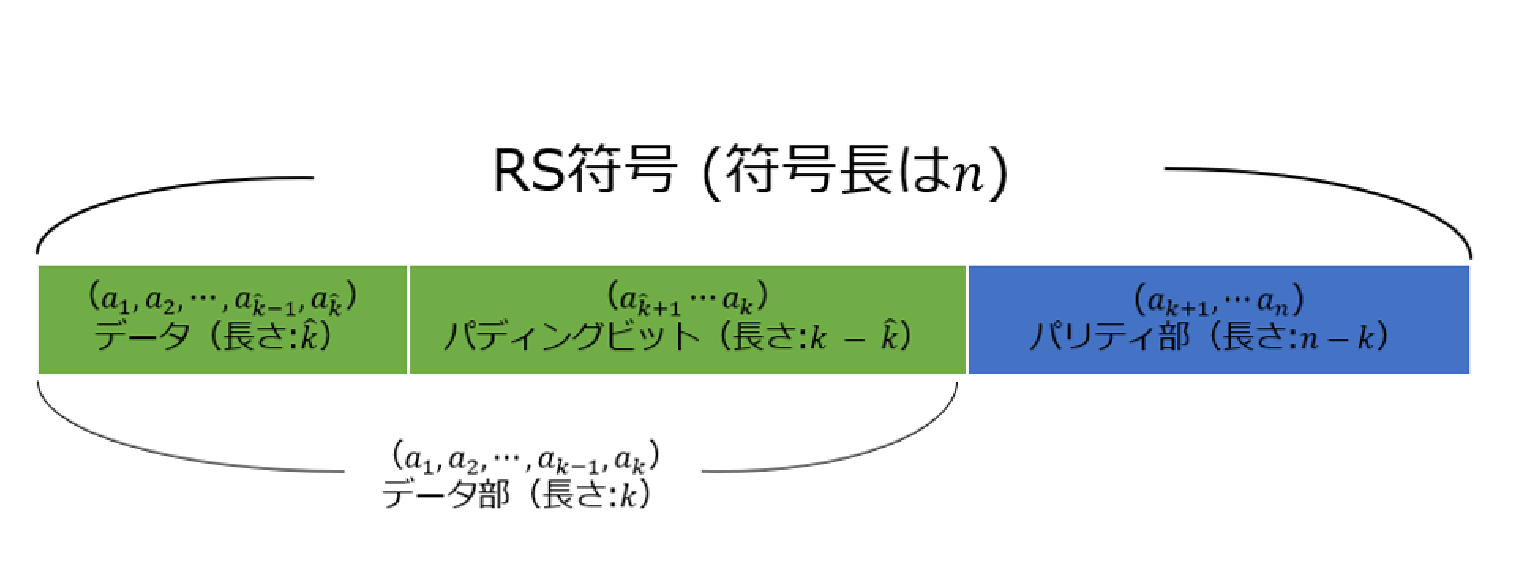
\includegraphics[width=1\linewidth]{pic/RScode.eps}
 \caption{RS符号の全体図\label{RScode}}
\end{figure}

パディングビットはQRコードに入力するデータとは関係ないため、自由に変更できる.
パディングビットを変更することにより、RS符号を形成する多項式の係数は変わる.
そのため、RS符号化で得られる符号の値も変化する.

\section{QRコードの概要}

QRコードの構成要素の最小単位は白と黒で表されるモジュールであり、各モジュールには単一ビット値が割り当てられる.
QRコードのサイズはバージョンによって決定され、そのバージョン($v$)は$1\sim40$である.
$1$型は、$21\times21$モジュール、$2$型は、$25\times25$モジュール、というように、型番が一つ上がるごとに一辺につき$4$モジュールずつ増加し、$40$型は、$177\times177$モジュールとなる.
したがって、バージョン$v$は$(17+4v)\times(17+4v)$モジュールである.

図\ref{fig:qrcode_config}にQRコードの構成要素を表す. \\

\begin{figure}[H]
\centering
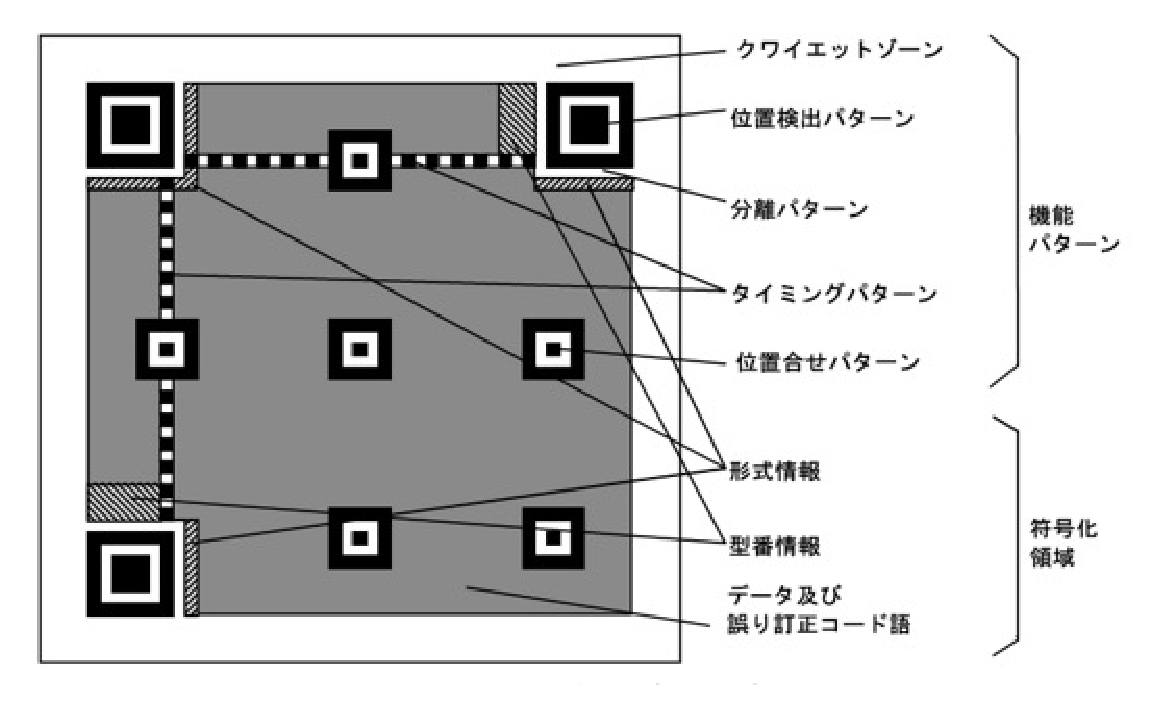
\includegraphics[width=10cm,clip]{pic/qrcode_config.eps}
\caption{QRコードシンボルの構造\cite{jis}}
\label{fig:qrcode_config}
\end{figure}

QRコードは、QRコード上にある符号化されたデータを正確に認識するために機能パターンを持っている.
機能パターンは主に3つの構成要素から成り立っており、それぞれ位置検出パターン、位置合わせパターン、タイミングパターンと呼ばれる.

位置検出パターンはQRコードの左上、左下、右上の角にある3つの正方形のブロックである.
それらの境目を明白にするために、形式情報との間に白いモジュールを置く.これを分離パターンと呼ぶ.

位置合わせパターンは小さな正方形のブロックで、位置検出パターンの垂直・平行座標に関係する位置に置く.バージョンによっては付加しない場合もあり、バージョン1には存在しない.

タイミングパターンは左上の位置検出パターンから右上の位置検出パターンへと、左上の位置検出パターンから左下の位置検出パターンへの白黒が交互に並ぶ$2$つのラインのことである.

QRコードのデータビットは、QRコードの右下から始まり、2モジュール幅の列上に配置する.列が最上部に達すると、次の2モジュール列は右端から始まり、下方向へ続く.現在の列が端に達すると、次の2モジュールの列に移動して方向を変更する.データビットは機能パターン(位置検出パターン、タイミングパターン、位置合わせパターン)の位置では、次のモジュールへ配置される.

上方向のデータビットの配置は表\ref{up_bit}に、下方向のデータビットの配置は表\ref{down_bit}に示す.

\begin{table}[h]
 %---- 最初の表 ---------------------------
  \begin{minipage}[t]{.45\textwidth}
    \begin{center}
	\caption{上方向のビット配列 \label{up_bit}}
      \begin{tabular}{|c|c|} \hline
	0&1\\ \hline
	2&3\\ \hline
	4&5\\ \hline
	6&7\\ \hline
      \end{tabular}
    \end{center}
  \end{minipage}
  %
  \hfill
  %
 %---- 2つ目の表 ---------------------------
  \begin{minipage}[t]{.55\textwidth}
    \begin{center}
	\caption{下方向のビット配列 \label{down_bit}}
      \begin{tabular}{|c|c|} \hline
	6&7\\ \hline
	4&5\\ \hline
	2&3\\ \hline
	0&1\\ \hline
      \end{tabular}
    \end{center}
  \end{minipage}
\end{table}

QRコードは、誤り訂正にRS符号を使用し、その能力はL、M、Q、Hの$4$つのレベルに昇順で分類される.
各誤り訂正レベルはQRコード内の全シンボルの約$7\%$、約$15\%$、約$25\%$、約$30\%$までのシンボルを訂正することができる.
それぞれを表\ref{Correction_ability}に示す.

\begin{table}[htbp]
\begin{center}
  \caption{誤り訂正レベル \label{Correction_ability}}
    \begin{tabular}{|c|c|c|c|c|} \hline
     レベル&L&M&Q&H\\ \hline\hline
     誤り訂正能力&約$7\%$&約$15\%$&約$25\%$&約$30\%$ \\ \hline
    \end{tabular}{}
\end{center}
\end{table}


%%%%%%%%%%%%%%%%%%%%%%%%%%%%%%%%%%%%%%%%%%%%%%%%%%%%%%%%%%%%%%%%%%%%%%%%%%%%%%%%%%%%%%%%%%%%%%%%%%%%%%%%%%%%%%%%%

\chapter{Aesthetic QRコード}

\section{色変換手法}
QRコードの標準形式にしたがって、各モジュールは基本的に黒と白で表現される.しかし、以下の理由によりモジュールに色を使用することは可能である.


\begin{algorithm}                      
\caption{論文\cite{KURI}の色変換手法}         
\label{alg:alg1} 
\begin{description}
\item[入力:] サイズ$L \times L$の目的画像
\item[出力:] 閾値 $\overline{Y}$
\item[方法:]
\begin{enumerate}
\item 入力画像の大きさは、QRコードのバージョン$v$と同じサイズに予め変更しておく.RGB色成分はYUV色成分に変換され、輝度(Y)成分$Y_{i,j}$,($1 \leq i,j \leq L$)が得られる.
\item その中心の正方形(元の画像サイズの$\frac{1}{4}$)の値の平均$\overline{Y}$が計算する.
\begin{equation}
\overline{Y} = \frac{4}{L^2} \sum_{i = \frac{L}{4}}^{\frac{3L}{4} - 1} \sum_{j = \frac{L}{4}}^{\frac{3L}{4} - 1} Y_{i,j}
\label{eq:pol4}
\end{equation}
\end{enumerate}
\end{description}
\end{algorithm}  


閾値を用いて目的画像から目的画像の二値行列を作成するアルゴリズムを以下に示す.

\begin{algorithm}                      
\caption{目的画像に紐づいた二値行列の生成}         
\label{alg:alg2} 
\begin{description}
\item[入力:] サイズ$L \times L$の目的画像の輝度(Y)成分$Y_{i,j}$($1 \leq i,j \leq L$)、閾値$A$
\item[出力:] 二値行列$B_{i,j}$
\item[方法:]
\begin{enumerate}
\item 目的画像を二値化する際、二値行列$B_{i,j}$は、以下の規則によって決定される.
\begin{equation}
{B_{i,j} =}
\begin{cases}
1 & Y_{i,j} > A \\
0 & otherwise 
\end{cases}
\label{eq:binary}
\end{equation}
\end{enumerate}
\end{description}
\end{algorithm} 

論文\cite{KURI}は二値行列$B_{i,j}$を求める際に式(\ref{eq:binary})の閾値$A$へ$\overline{Y}$を代入する.


\section{ランダム法}
ここにランダム法の説明を書く(これより前の章でRS符号の符号化を説明しないといけない)

QRコードを作成する手順を以下に説明する.

\begin{algorithm}                      
\caption{論文\cite{KURI}のランダム法}         
\label{alg:alg3} 
\begin{description}
\item[入力:] バージョン$1$のQRコードに入る範囲内の文字列、かつサイズ$21 \times 21$の目的画像
\item[出力:] サイズ$21 \times 21$のバージョン$1$のQRコード
\item[方法:]
\begin{enumerate}
\item
目的画像の画素値をQRコードのモジュールに割り当て、Algorithm2で決まった閾値$\overline{Y}$でモジュールを二値化し、二値行列$B_{i,j}$を作成する.
\item
$B_{i,j}$に所定のマスキングパターンを作用させる.
\item
式(\ref{eq:pol3})の$\alpha_{x_t}$($\hat{k} + 1 \leq x_t \leq k $)を変化させることにより、$B_{i,j}$とのハミング距離が最小となるRS符号を見つける.以後この手順を$N$回繰り返すことにより、最良のRSブロックの組を決める.
一定の試行回数終了後、QRコード上RS符号は、最良のRS符号$\alpha_{x_t}$に置き換える.
\item
マスク処理前であるQRコードの各モジュールに対して、所定のマスクパターンを適用する.
\end{enumerate}
\end{description}
\end{algorithm} 
これにより、サイズ$21 \times 21$のQRコードを作成する.

%%%%%%%%%%%%%%%%%%%%%%%%%%%%%%%%%%%%%%%%%%%%%%%%%%%%%%%%%%%%%%%%%%%%%%%%%%%%%%%%%%%%%%%%%%%%%%%%%%%%

\chapter{実験}

この章では

\section{実験環境}

実験に使用したPC環境、言語を以下に示す.

\begin{itemize}
\setlength{\itemsep}{5mm}
 \item ソフトウェア実装環境
    \begin{itemize}
      \item CPU:Intel(R)Core(TM) i7-7700 CPU @ 3.60GHz 3.60GHz
      \item OS:Windows 10 pro
      \item 実装RAM:16.0GB
     \end{itemize}
   \item 開発環境
    \begin{itemize}
      \item Java:Eclipse 4.11.0
      \item Maple:Maple 2017.3
   \end{itemize}
\end{itemize}

実験に使用した各パラメータを以下に示す.

\begin{itemize}
\setlength{\itemsep}{5mm}
 \item QRコード
    \begin{itemize}
      \item 入力文字:FUKUDA
      \item バージョン$(v)$:$1$
      \item マスクパターン:$001$
      \item 誤り訂正レベル:M
     \end{itemize}
  \end{itemize}

%%%%%%%%%%%%%%%%%%%%%%%%%%%%%%%%%%%%%%%%%%%%%%%%%%%%%%%%%%%%%%%%%%%%%%%%%%%%%%%%%%%%%%%%%%%%%%%%%%%%

\chapter{結果}


\section{評価}

画像の評価は
\begin{enumerate}
\item
目的画像の二値行列$B_{i,j}$と得られたQRコードの二値行列におけるハミング距離の総数
\item
$MSE$(平均二乗誤差)
\item
$PSNR$(ピーク信号対雑音比)
\end{enumerate}
で行う.

\subsection{最小ハミング距離}

2つの符号語つの符号語$a=(a_1,a_2,…,a_n)$と$b=(b_1,b_2,…,b_n)$で対応するビット(桁)で値$(0$または$1)$が異なっているビット(桁)の数をハミング距離と言い、記号で$d(a,b)$と書く.
その中でも一番ハミング距離が小さいものを最小ハミング距離と呼ぶ.

ハミング距離は2つの符号語$a=(a_1,a_2,…,a_n)$と$b=(b_1,b_2,…,b_n)$に対して以下の式で定義される.

\begin{eqnarray}
d(a,b)=\sum_{i=1}^{n}(a_{i}+b_{i})\mbox{ }(\mbox{mod } 2)
\end{eqnarray}


\subsection{$MSE$(平均二乗誤差)}

$MSE$は元画像と処理画像との差の2乗誤差である.$MSE$が小さければ小さいほど元画像に近い画像である.
$MSE$は$M \times N$の2つの画像$I、K$において、以下の式で定義される.

\begin{eqnarray}
MSE&=&\frac{1}{MN}\sum_{i=0}^{M-1}\sum_{j=0}^{N-1}[I(i,j)+K(i,j)]^2
\end{eqnarray}


\subsection{$PSNR$(ピーク信号雑音比)}

$PSNR$は画質の再現性に影響を与える信号がとりえる最大の輝度と劣化をもたらすノイズの比率を示したものである.
$PSNR$は以下の式で定義される.

\begin{eqnarray}
PSNR&=&10\log{10}\frac{MAX_I^2}{MSE} \\
       &=&20\log{10}\frac{MAX_I}{\sqrt{MSE}}
\end{eqnarray}

$MAX_{I}$は画像がとりうる最大ピクセルを表す.
ピクセルの$1$サンプルが$8$ビットで表現されている場合、$MAX_{I}$は$255$である.

画質の評価については以下に示す.
実際にソフトウェアによって生成した画像が図\ref{fig:nomal}$\sim$図\ref{fig:output_10000}である.
\begin{figure}[H]
  \begin{tabular}{cc}
    %---- 最初の図 ---------------------------
    \begin{minipage}[t]{0.45\hsize}
      \centering
      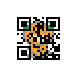
\includegraphics[width=0.5\linewidth]{pic/nomal.eps}
      \caption{従来の方法で作成したAesthetic QRコード}
      \label{fig:nomal}
    \end{minipage} &
    %---- 2番目の図 --------------------------
    \begin{minipage}[t]{0.45\hsize}
      \centering
      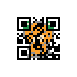
\includegraphics[width=0.5\linewidth]{pic/output_1.eps}
       \caption{$N=1$}
      \label{fig:outuput_1}
      \end{minipage}
  \end{tabular}
\end{figure}

 %---- 改行 ----------------------

\begin{figure}[H]
  \begin{tabular}{cc}
    %---- 3番目の図 ---------------------------
    \begin{minipage}[t]{0.45\hsize}
      \centering
      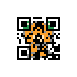
\includegraphics[width=0.5\linewidth]{pic/output_10.eps}
       \caption{$N=10$}
      \label{fig:output_10}
    \end{minipage} &
    %---- 4番目の図 --------------------------
    \begin{minipage}[t]{0.45\hsize}
      \centering
      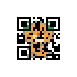
\includegraphics[width=0.5\linewidth]{pic/output_100.eps}
      \caption{$N=100$}
      \label{fig:output_100}
      \end{minipage}
  \end{tabular}
\end{figure}

 %---- 改行 ----------------------

\begin{figure}[H]
  \begin{tabular}{cc}
    %---- 5番目の図 ---------------------------
    \begin{minipage}[t]{0.45\hsize}
      \centering
      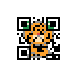
\includegraphics[width=0.5\linewidth]{pic/output_1000.eps}
       \caption{$N=1000$}
      \label{fig:output_1000}
    \end{minipage} &
    %---- 6番目の図 --------------------------
    \begin{minipage}[t]{0.45\hsize}
      \centering
      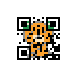
\includegraphics[width=0.5\linewidth]{pic/output_10000.eps}
       \caption{$N=10000$}
      \label{fig:output_10000}
      \end{minipage}
  \end{tabular}
\end{figure}
  %---- 図はここまで ----------------------


目的画像の二値行列$B_{i,j}$と得られたQRコードの二値行列とのハミング距離の総和は表\ref{tab:Haming}に示す.

\begin{table}[H]
	\caption{目的画像の二値行列$B_{i,j}$と得られたQRコードの二値行列とのハミング距離の総和}
	\begin{center}
  		\begin{tabular}{|c|c|c|c|c|c|c|} \hline
     			生成した回数 $(N) $& $従来の生成方法$ & $1$ & $10$ & $100$ & $1000$ & $10000$  \\  \hline
   			最小ハミング距離 & $79$& $83$ & $69$ & $67$ & $53$ & $47$\\ \hline
     		\end{tabular}
  	\end{center}
  \label{tab:Haming}
\end{table}
 
ランダム法の$MSE$値を表\ref{tab:MSE}に示す

\begin{table}[H]
	\caption{ランダム法の$MSE$値}
	\begin{center}
  		\begin{tabular}{|c|c|c|c|c|c|c|} \hline
     			生成した回数 $(N) $& $従来の生成方法$ & $1$ & $10$ & $100$ & $1000$ & $10000$  \\  \hline
   			$MSE$値 & $24110.33$& $25075.25$ & $23874.78$ & $23680.28$ & $21961.52$ & $21490.57$\\ \hline
     		\end{tabular}
  	\end{center}
  \label{tab:MSE}
\end{table}


ランダム法の$PSNR$値を表\ref{tab:PSNR}に示す

\begin{table}[H]
	\caption{ランダム法の$PSNR$値}
	\begin{center}
  		\begin{tabular}{|c|c|c|c|c|c|c|} \hline
     			生成した回数 $(N) $& $従来の生成方法$ & $1$ & $10$ & $100$ & $1000$ & $10000$  \\  \hline
   			$PSNR$値$(dB)$ & $31.89$& $31.50$ & $31.99$ & $32.07$ & $32.82$ & $33.04$\\ \hline
     		\end{tabular}
  	\end{center}
  \label{tab:PSNR}
\end{table}

\acknowledgement

お礼を書きます.

\begin{thebibliography}{99}

%
\bibitem{QR}
QR code.com. http://www.qrcode.com/en.
%
\bibitem{hist}
Visualead. http://www.visualead.com.
%
\bibitem{KURI}
M. Kuribayashi and M . Morii "Aesthetic QR Code Based on Modified Systematic Encoding Function",
IEICE transactions on information and systems ,VOL.E100–D, NO.1,pp.42-51,2017.
%
\bibitem{jis}
JIS X0510. http://www.jisc.go.jp/app/pager?id=2738494. 
\end{thebibliography}

\appendix

\chapter{その他}

ここでは番号がすべてアルファベットに変わります.

\end{document}


